\documentclass{report}

\usepackage{pgfplots}
\pgfplotsset{compat=1.18}
\usepackage{tikz}
    \usetikzlibrary{arrows.meta}

\graphicspath{{figures/}}

\begin{document}
\section{Coordinates}
\begin{figure}[!h]
\centering
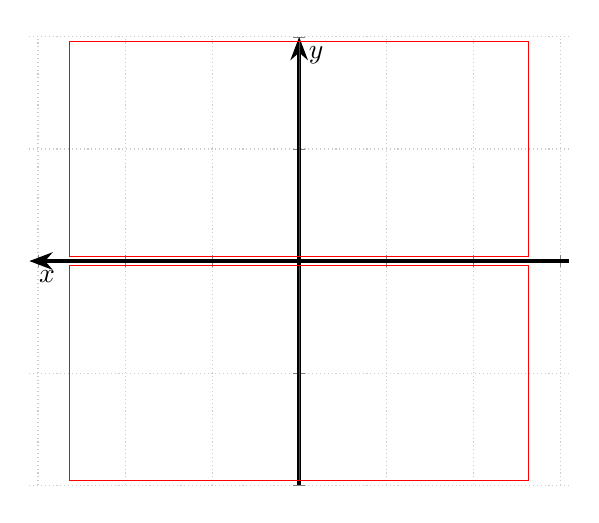
\begin{tikzpicture}
    \def\x{13.19};
    \def\y{9.8};
    \begin{axis}[
	axis lines = middle,
	axis line style = {-Stealth, very thick},
	xmin = -15.5, xmax = 15.5, ymin = -10, ymax = 10,
	x dir = reverse,
	% xtick distance = 1,
	% ytick distance = 1,
	xticklabel = \empty,
	yticklabel = \empty,
	xlabel = $x$,
	xlabel style = { at = {(current axis.left of origin)}, anchor = south west, below right},
	ylabel = $y$,
	grid = major,
	grid style = {thin, densely dotted, black!20} ]
	\draw[red] (0,  0.2) rectangle ( \x,  \y);
	\draw[red] (0,  0.2) rectangle (-\x,  \y);
	\draw[red] (0, -0.2) rectangle ( \x, -\y);
	\draw[red] (0, -0.2) rectangle (-\x, -\y);
    \end{axis}
\end{tikzpicture}
\end{figure}


\section{Cable connection}
\begin{figure}[h]
    \centering
    \includegraphics[width=0.49\linewidth]{hexBoard}
    \includegraphics[width=0.49\linewidth]{sqaBoard}
\end{figure}

Relative position (w.r.t. the bottom right of the PCB) of each SiPM (top down):

Hex board (x, y):
\begin{itemize}
    \item top middle: (50.01 mm, 80.90 mm)
    \item top left:   (77.64 mm, 64.95 mm)
    \item top right:  (22.37 mm, 64.95 mm)
    \item middle middle: (50.01 mm, 48.99 mm)
    \item bottom left: (77.64 mm, 33.04 mm)
    \item bottom right: (22.37 mm, 33.04 mm)
    \item bottom middel: (50.01 mm, 17.08 mm)
\end{itemize}

Sqa board (x, y):
\begin{itemize}
    \item top left: (73.9 mm, 72.89 mm)
    \item top right: (26.1 mm, 72.89 mm)
    \item bottom left: (73.9 mm, 25.09 mm)
    \item bottom right: (26.1 mm, 25.09 mm)
\end{itemize}

\subsection{Abnormal boards}
\begin{itemize}
    \item L3:B25 -- hexagonal, left, channel 0--6, top down
	\begin{figure}[h]
	    \centering
	    \includegraphics[scale=0.025]{board25_back}
	    \includegraphics[scale=0.025]{board25_front}
	\end{figure}
    \item L3:B28 -- hexagonal, right, channel 0-6, top down
	\begin{figure}[h]
	    \centering
	    \includegraphics[scale=0.025]{board28_back}
	\end{figure}
    \item L4:B41 -- square, left, channel 0-3, top down
    \item L4:B37 -- hexagonal, right, channel 0-3, top down
	\begin{figure}[h]
	    \centering
	    \includegraphics[scale=0.025]{board37_back}
	    \includegraphics[scale=0.025]{board37_front}
	\end{figure}
    \item L5:B38 -- square, right, channel 0-3, top down
	\begin{figure}[h]
	    \centering
	    \includegraphics[scale=0.025]{board38_front}
	\end{figure}
    \item L5:B21 -- square, left, channel 0-3, top down
	\begin{figure}[h]
	    \centering
	    \includegraphics[scale=0.025]{board21_back}
	\end{figure}
    \item L5:B18 -- square, right, channel 0-3, top down
	\begin{figure}[h]
	    \centering
	    \includegraphics[scale=0.025]{board18_back}
	    \includegraphics[scale=0.025]{board18_front}
	\end{figure}
    \item L8:B15 -- square, left, channel 0-3, top down
	\begin{figure}[h]
	    \centering
	    \includegraphics[scale=0.025]{board15_front}
	    \caption{Board 15}
	\end{figure}
    \item L8:B46 -- square, left, channel 0-3, top down
	\begin{figure}[h]
	    \centering
	    \includegraphics[scale=0.025]{board46_back}
	\end{figure}
    \item L9:B20 (L9:B45, L10:B49, L11:B52, L11:B19) -- square, left, channel 0-3, top down
	\begin{figure}[h]
	    \centering
	    \includegraphics[scale=0.025]{board20_back}
	    \includegraphics[scale=0.025]{board20_front}
	\end{figure}
    \item L10:B16 -- square, right, channel 0-3, top down
	\begin{figure}[h]
	    \centering
	    \includegraphics[scale=0.025]{board16_back}
	    \includegraphics[scale=0.025]{board16_front}
	\end{figure}
\end{itemize}
\end{document}
